\documentclass[10pt,letterpaper]{article}

\usepackage{graphicx}
\usepackage{url}
\usepackage{color}
\usepackage{ifpdf}
\usepackage{wrapfig}
%\usepackage[cm]{fullpage}
\usepackage{textcomp}
\usepackage{srcltx}
\usepackage{fancyhdr}
\usepackage{setspace}
\usepackage{subfigure}

% Space saving
\usepackage[small,compact]{titlesec}
\usepackage[small,it]{caption}

\renewcommand\floatpagefraction{.9}
\renewcommand\topfraction{.9}
\renewcommand\bottomfraction{.9}
\renewcommand\textfraction{.1}
\setcounter{totalnumber}{50}
\setcounter{topnumber}{50}
\setcounter{bottomnumber}{50}

% set left and right margin, and top margin
%\setlength{\topmargin}{0cm}
%\setlength{\headheight}{0cm}
%\setlength{\headsep}{0cm}
%\setlength{\oddsidemargin}{0cm}
%\setlength{\evensidemargin}{0cm}

\textwidth = 6.5315 in
\textheight = 9.0315 in
\oddsidemargin = 0.0 in
\evensidemargin = 0.0 in
\topmargin = 0.0 in
\headheight = 0.0 in
\headsep = 0.0 in
\parskip = 0.056in
\parindent = 0em
% \parskip = 0.0716in
% \parindent = 0.0cm
\textfloatsep = 0.1in


\ifpdf \pdfinfo{ /Author (Shantenu Jha et al.)  /Title (SAGA: A
  Critical Abstraction Layer for Distributed Applications and
  Systems)}

  \usepackage[pdftex,colorlinks=true, linkcolor=blue,citecolor=blue,
       urlcolor=blue]{hyperref}
\else
  \usepackage{hyperref}
\fi

\graphicspath{{figures/}{../figures}}

\newcommand{\projectname}{\textit{SAGA}}
\newcommand{\productname}{\textit{SAGA-GridSAT}}
\newcommand{\firstprincipleapplication}{\textit{Kalman-Filter}}
\newcommand{\ci}{{cyberinfrastructure }}

%\newcommand{comment#1{{\textcolor{magenta}#1}}

\newcommand{\projectnamefull}{\textit{SAGA: A Strategic
    Advancement for Grid Applications } }

\newcommand{\upup}{\vspace*{-0.5em}}
\newcommand{\upp}{\vspace*{-0.5em}}
\newcommand{\up}{\vspace*{-0.25em}}

\newcommand{\mywp}[2]{
  \hline
  \multicolumn{2}{|c|}{
    \rule[-.5em]{0em}{2em}
    \B{\large Work Package #1:}{\large #2}
  }\\
}

\newcommand{\mytask}[1]{
  \multicolumn{2}{|l|}{
    \rule[-.8em]{0em}{2em}
    \I{\large #1}
  }\\
}

\ifpdf
  \DeclareGraphicsExtensions{.pdf, .png}
\else
  \DeclareGraphicsExtensions{.ps, .eps}
\fi

\begin{document}

%\long\def\comment#1{{\textcolor{magenta}#1}}
\long\def\comment#1{{\bf \textcolor{magenta}{\bf #1}}}
\long\def\ccomment#1{{\bf \textcolor{blue}{\bf #1}}}
\newcommand{\C}{\comment}
\newcommand{\CC}{\ccomment}
%\newcommand{\C}[1]{}
%\newcommand{\CC}[1]{}
%\newcommand{\F}[1]{}

%\newcommand{\assign}[1]{\small \textcolor{magenta}{#1}}
\newcommand{\assign}[1]{}

\newcommand{\I}{\textit}
\newcommand{\B}{\textbf}
\newcommand{\T}{\texttt}
\newcommand{\F}[1]{\B{\textcolor{red}{FIXME: #1}}}

\newenvironment{shortlist}{
        \vspace*{-0.9em}
  \begin{itemize}
  \setlength{\itemsep}{-0.5em}
}{
  \end{itemize}
        \vspace*{-0.8em}
}

\newenvironment{shorttablelist}{
        \vspace*{-0.4em}
  \begin{itemize}
  \setlength{\itemsep}{-0.3em}
}{
  \end{itemize}
        \vspace*{-1.6em}
}

% turn off indentation completely
\setlength{\parindent}{0mm}
\addtolength{\parskip}{-.25em}

\newif\ifdraft
%\drafttrue
\ifdraft
 \newcommand{\jhanote}[1]{  {\textcolor{red}    { ***Shantenu: #1 }}}
 \newcommand{\katznote}[1]{ {\textcolor{cyan}   { ***Dan:      #1 }}}
 \newcommand{\amnote}[1]{   {\textcolor{magenta}{ ***Andre:    #1 }}}
 \newcommand{\hknote}[1]{   {\textcolor{blue}   { ***Hartmut:  #1 }}}
\else
 \newcommand{\jhanote}[1]{}
 \newcommand{\katznote}[1]{}
 \newcommand{\amnote}[1]{}
 \newcommand{\hknote}[1]{}
\fi

%\newcommand{\hknote}[0]{}

\pagestyle{fancy} 
\pagenumbering{arabic} 
\fancyhead{}
\fancyfoot{}

\lfoot{\footnotesize \projectname:\ Page \thepage}

\setcounter{subsection}{0}

\pagestyle{empty}

\setcounter{page}{1}
\pagestyle{plain} 
\normalsize
%\section{Introduction}

\section{Project Overview and Description}

Although \ci has matured considerably over the past few years,
applications that can effectively utilize these technologies are far
from ubiquitous.  Advances in distributed application have simply not
kept pace with advances in other aspects of distributed
cyberinfrastructure (CI). This is true whether measured by the number
of \I{novel} applications developed to exploit the infrastructure, or
even something simpler, such as the number of applications that can
utilize multiple resources to reduce the time-to-solution of
scientific problems.
% measured by the number of existing applications that can easily
% utilize the many \I{advanced} features offered by distributed
% infrastructure or.
A key impediment in the accelerated development and deployment of
distributed applications is the scarcity of high-level 
programming abstractions and interfaces that bridge the divide
between the needs of distributed applications and the capabilities
offered by middleware and system-level
interfaces~\cite{cloud-saga-paper}.

\jhanote{introduce imbalance in cyberinfrastructure here again; reduce
  time to solution using distributed infrastructure}
\jhanote{Distributed systems exist as production systems,
  unfortunately not for applications}

In general, applications that are able to leverage the heterogeneity
and dynamic performance response inherent in the Grid, to their
advantage, have proved exceedingly difficult to implement.  Much
development has focused on the support for legacy parallel and cluster
applications codes, without changing application usage and execution
modes.  In part, this is also due to a lack of suitable abstractions
to re-architect ``legacy applications'' to have agile execution and
usage modes, as well as to develop ``first principles'' distributed
applications.  There exist an unexplored range of applications that
can benefit from the Grid paradigm; progress on this front will come
from application development that does not depend on the homogeneous,
isolated and relatively static model of resource allocation and
performance inherited from parallel or cluster legacies.  In many
ways, the current situation is analogous to that which existed when
vector processing hardware was introduced.  Scientific codes written
for previous architectures could be ported to vector machines, but the
true power of the approach was only available to hand-coded ``assembly
language'' examples that could directly exploit the vector hardware
and memory model.  Until codes were re-written and new codes developed
specifically with vectorization in mind, the performance benefits were
not fully realized.


% Another way in which distributed application development is being
% retarded by a lack of suitable abstractions is inability to
% re-architect ``legacy applications'' to have agile execution and usage
% modes, as well as in the development of ``first principles'' Grid
% applications.

The lack of such application-level programming abstractions is
compounded by the fact that there exist often incompatible middleware
systems in both research and production environments.  There are
efforts~\cite{gin-bes-hpc} to harmonize different Grids by using a
medley of tools, inter-operational efforts and standardization in the
many layers \I{below the application level}.  Although driven with the
noble aim of increasing the utilization of Grids, their impact in
facilitating applications remains unclear; these are likely to be
necessary steps towards effective distributed systems, but not
sufficient.

To address these challenges and in particular to find a solution to
the universal, apparently intractable problem of successfully enabling
applications to utilize multiple, distributed resources seamlessly,
several applications groups expressed the desire for a simple
programmatic interface that is widely-adopted and available.  The goal
of such an interface would be to provide a ``grid counterpart to MPI''
(at least in impact if not in details) and that would supply
developers with a simple, uniform, and standard programmatic interface
with which to develop applications.  Thanks to the efforts of many
contributors, but in particular the efforts of the PI's group, an
initial specification of such a ``grid counterpart to MPI'' now exists
-- the Simple API for Grid Applications (SAGA)~\cite{saga-core}. SAGA
is an Open Grid Forum (OGF)~\cite{ogf} proposed recommendation on the
path to becoming a standard.  The need now is to demonstrate the
unique benefits of adopting the SAGA paradigm by delivering concrete
examples of advanced Grid applications.

% This is representative of the near universal support for SAGA, and
% agreement on its critical role in facilitating the development of Grid
% applications (see letters of support).  

We have recently demonstrated the power of this approach in two
distinct but powerful ways. In the first, we re-architected an
application-based upon Kalman-filters and applied to reservoir
simulations, to have an agile execution model capable of utilizing
several resources on the TeraGrid. The coding of the application
using SAGA was the single important feature which endowed an otherwise
well-known ``legacy'' application with a novel dynamic execution
mode. Specifically, SAGA was used to determine at run-time, via
BQP~\cite{bqp} the optimal resource to launch sub-tasks dynamically,
and be able to exploit multiple resources concurrently without prior
negotiation or requirement analysis. Recognizing the potential impact
of this approach, our paper describing and demonstrating this work was
awarded the Performance Challenge award held at TeraGrid 2008
Conference, Las Vegas\footnote{Performance Challenge Award, TeraGrid
  2008, Las Vegas,
  \url{http://www.tacc.utexas.edu/tg08/index.php?m_b_c=awards}}. We
have also shown how another legacy application (NAMD~\cite{NAMD}),
when used to implement common algorithms such as Replica-Exchange on
multiple distributed infrastructure, can have a simple, yet very
impactful difference. By using SAGA to present a uniform and unified
resource access mechanism, the greater the number of distributed
resources employed, less was the time-to-solution~\cite{saga_papers}. 
It is critical to understand that
SAGA is not middleware but a distributed programming abstraction layer
that is aimed directly at application uptake of Cyberinfrastructure,
and making it both easier and more productive for scientists to
utilize CI.  We will present in Section~\ref{saga-apps}, greater
details of the scientific applications and advances possible by novel
usage and execution modes that are made possible by SAGA.  \amnote{gap
  above} \jhanote{you mean ``mind the gap''?}

%all that is required from the end-user/application developer is to
%codify their application using SAGA. 

Interestingly, a well defined and established
taxonomy of distributed applications does not exist. The PI in recent work, along
with collaborators has been developing the first comprehensive
taxonomy of distributed applications, based upon real scientific
distributed applications and an analysis of their
characteristics~\cite{dpa-paper, dpa-wiki}.  Based partially upon this
taxonomy, we outline three categories of distributed applications that
we have already developed using SAGA: (i) Legacy applications where
either local functionality is swapped for distributed functionality,
(for example, distributed replica exchange of simulations), or where
distributed execution models are provided~\cite{saga_tg08}; (ii)
Applications based upon frameworks that are developed using
SAGA. There are multiple examples of successful applications that use
this approach, such as MapReduce, All-Pairs, and migrating
applications. Typically, the computational logic here is well
separated from the distributed logic; the application is unaware of
the distribution environment, while the framework contains the
distributed logic, and (iii) First principles distributed applications
(such as adaptive applications~\cite{saga_escience07}) where
scientific applications are explicitly cognizant of the fact that they
will operate in a distributed environment and the computational logic
is coupled with the distributed logic.

In this work we propose to develop, using SAGA as the basis, the
programming abstractions necessary to support distributed applications
of all three types and to make those abstractions available to the
TeraGrid, and to the wider community.  We will validate and extend
SAGA so that it can support the development of the spectrum of
application classes -- from the exotic dynamically adaptive and
self-reconfiguring functionality that is necessary to exploit a
heterogeneous and constantly-changing resource pool, to the {\it
  mundane} parameter-sweep which utilizes multiple resources but does
this under the covers.  \B{The overall goal of this effort is to make
  SAGA in its enhanced form available to the wider TeraGrid
  application and development community, as a vehicle for providing
  legacy applications with new usage modes to utilize distributed
  infrastructure, to stimulate the development of new applications
  that target a distributed execution platform explicitly and to
  provide a balanced cyberinfrastructure from the perspective of
  broad-range of scientific applications.}

%leverage significant investments in the TeraGrid
% To drive this development...  ...  as a primary motivating and
% verifying application.  .. to its performance advantage and it has
% successfully combined production resources from multiple TeraGrid
% sites to generate new scientific results

% Our plan is to use our experience with a myriad of applications to
% inform the extension of SAGA so that it can support the next
% generation of distributed applications that will share agile execution
% models.  We will also establish how support for an agile execution
% model at the programming level will impact \I{legacy} (statically
% distributed) scientific applications. Specifically, we will marshal
% resources and coordinate the distributed functionality (i.e.,
% implement the distributed logic) of replica-exchange type simulations using
% SAGA and demonstrate, (i) how interoperability across Grid arises
% automatically as a consequence and, (ii) how larger and more
% meaningful biophysical models can be investigated. 

\B{SAGA: Using Cyberinfrastructure via a high-level distributed
  Programming Interface}: Although it may not be normal practice, we
believe circumstances warrant a quote from the panel summary of our
previous (unsuccessful) STCI submission: ``The panel recognizes the
importance of the CI problem addressed by the proposed effort. Making
it easier for applications to harness the power of distributed
computing resources is of great interest to the community.''  We would
like to concur with the panel, in that we believe that the single
important and fundamental challenge in CI is reducing the barrier for
scientific application development, deployment and effective uptake of
infrastructure. To achieve this, it is critical to provide the right
abstractions at the application level, to enable applications to be
developed independent of the specifics of middleware distributions
and, applications once developed, must remain immune to the evolution
and dynamics of diverse CI environments.  Effective application
development requires \I{simple} interfaces to allow \I{uniform} access
to the different Grid functionalities which must be \I{stable}
(i.e. new versions are compatible with existing code) and \I{easy} to
deploy and use at runtime.  CI environments are built on a variety of
hardware and software architectures and thus applications need to be
\I{portable}, and hence require implementations that provide these
features over a range of platforms.  Additionally, any such
programming interface should cover a broad range of different
programming paradigms and usage scenarios and therefore should not be
restrictive.  SAGA addresses these challenges by providing a
programming interface that integrates the most common programming
abstractions while respecting critical {\it application} level
requirements, namely, those of simplicity, stability, portability, and
uniformity.  SAGA is designed with the fundamental aim of enabling
applications to utilize distributed CI, by providing a high-level,
semantically consistent programming abstraction which provides a
uniform interface to distinct flavors and versions of middleware
distributions. 

% GridSAT is also a highly specialized, carefully programmed, complex
% application.  Our intention when developing it was to test the limits
% of what was possible without regard for extensibility,
% maintainability, packaging for re-use, etc.  Metaphorically, we wanted
% to experiment with the ``assembly language programming'' of
% cyberinfrastructure to determine how effective an adaptive,
% autonomous, and dynamically self-reconfiguring application could be.
% Having proved the principle, we are now faced with the difficulty of
% generalizing the results and making the code available to the wider
% SAT community.  Doing so with the current GridSAT code base has proved
% a more daunting challenge than we have been able to overcome.  Our
% goal in developing a port of GridSAT to SAGA is both to test SAGA's
% ability to implement non-legacy, next-generation cyberinfrastructure
% applications, but also to provide a version of GridSAT that is more
% portable, extensible, and standards based than the current specialized
% (albeit successful) implementation.

% The overarching purpose of this proposal is to deliver an
% object-oriented programming environment to the TeraGrid community that
% is well-suited to the next generation of first principles Grid
% development.  SAGA will be used in other contexts but our intent with
% this work is to develop it into a complete set of abstractions that
% enable fully autonomous and adaptive Grid programs {\em without}
% burdening the programmer with tedious and error prone development
% activities.

% A direct outcome of the SAGA-GridSAT work, will be that extensions to
% the SAGA interface that will enable applications that have been
% traditionally distributed in a static fashion to exploit the dynamic
% and resource-aware features that enabled by SAGA. In particular,
% Replica-Exchange (RE) simulations using either Monte-Carlo (MC) or
% Molecular Dynamics (MD) will not longer have to be run on HPC Grids as
% batch jobs -- an execution model which does little to take cognizance
% of the fact that the length of simulations, number of replicas
% required and exchange attempt frequency is best left as a run-time
% variable, rather than a priori rigidly imposed variable.  Physical
% algorithms that can effectively utilize distributed computing
% infrastructure are often different from that those that utilize
% canonical high-end computers.  Replica exchange (RE) methods are a
% class of algorithms that can naturally utilize distributed computing
% infrastructure to understand physical properties of biomolecules.  RE
% approaches have, however, either been limited by the implementation
% (and thus the size and scale of the platforms used) or the execution
% model; consequently, only small physical systems have been
% investigated using these approaches so far.  By using existing
% community MD codes (such as NAMD or GROMACS) in an unmodified fashion,
% we will implement the distributed logic of a replica-exchange
% simulation using SAGA, which enables an agile execution model.  This
% \I{simple} software infrastructure will enables the use of RE
% methods to simulate large physical systems using HPC Grids.

\subsection*{Project Plan, Impact and Validation:}

\I{Core SAGA Effort (WP-1, 2 and 5)} involves all three phases of design,
development and deployment. In the design phase we will work to
provide extensions to existing interfaces; in the development phase
there will be effort at the both the engine and adaptor
levels. Finally we will work with regional CI (LONI and SURAgrid) and
national CI to ensure application-level interoperability on production
environments.

It is important to emphasis that several components of the SAGA
landscape already exist, for example an
implementation of the core C++ library; but many components currently
exist, if at all, mostly in a rudimentary form, and at best at the
level of research prototype.  The plan is to validate and harden
existing infrastructure, so as to move from research prototypes to
production grade infrastructure.

% \jhanote{ \begin{itemize}
% \item Design: new interfaces/packages and verification/validation \upp
% \item Development: Engine and other adaptors \upp
% \item Deployment: Testing harness, automatic updates, deployment on TG \upp
% \end{itemize} Say Core SAGA efforts are encompassed in WP-1-4..}

% \jhanote{Need to show that .
%  \begin{itemize}
% \item Frameworks to support Application Patterns \upp
% \item Managers.. \upp
% \item Others? \upp
% \end{itemize} }

\I{Impact on Real Scientific Applications (WP-4): } The application
suite in Table~\ref{appsuite} has been chosen based upon careful
theoretical studies and covers nearly all classes of distributed
applications. The set of applications chosen are also well-suited to
SAGA's interface and design and will benefit immediately from many of
existing functionality and interfaces that SAGA offers. This will
prepare the specific application for real science-production usage,
and in so doing provide validation of SAGA's current implementation
quality with respect to the TeraGrid. We believe the suite of
applications provide a minimally complete set of applications to be a
driving force to enable, validate, and extend SAGA on the TeraGrid.

\I{Education, Outreach and Training (WP-6):} In order to ensure far-reaching
impact we will develop SAGA tutorials, user documentation and
manuals.  The preparation of SAGA educational material requires
small effort, relative to the specification and implementation phase, 
but will go a long way in facilitating uptake of SAGA for legacy and
novel applications.  We will use the Louisiana Optical Network
Initiative (LONI) community and support structure for outreach and
training as we develop this, and then TeraGrid support for broader
outreach across the nation. 

Although portrayed as three different components of core development,
applications and EOT, in practice these efforts will be intertwined.
On the one hand SAGA needs enhancements at several levels (eg engine,
adaptor loading) so as to be easily deployable and usable before being
taken up by a wide application community, while on the other hand,
SAGA needs usage, uptake and engagement with user community in order
to reach the desired level of maturity and performance.

% \jhanote{Not sure: In practice any one applications will use efforts
%   in all three categories! For example, use SAGA to provide the
%   necessary encapsulation and uniformity across different middleware
%   flavors and distribution, but the heterogeneity of Grids need to be
%   addressed at some level (any level but the application level!). Thus
%   for any application to be deployed pervasively, requires supporting
%   software to be also deployed pervasively.  We plan to develop the
%   appropriate SAGA adaptors to bind SAGA to middleware and work with
%   the TeraGrid integration team to deploy them. We will also work in
%   conjunction with the GIN Community-Group~\cite{gin_url} to
%   demonstrate application-level interoperability~\cite{saga_gin07}. }

% Thus we believe that SAGA is the most-comprehensive,
% general-purpose attempt at providing such an application-level
% interface, and thus, 

\B{Impact:} From an applications perspective some measures of success
of CI include the number, the types of applications deployed and their
usage/execution modes supported by the distributed infrastructure.
SAGA is arguably the only application-level abstraction which
facilitates all three metrics.  This forms the core of our claims that
a stable, pervasive implementation and deployment of SAGA is
\I{strategically} very important in order to facilitate development of
current and the next generation cyberinfrastructure applications. This
proposal aims to put the full weight of SAGA behind a balanced CI from
an applications perspective.

% as well as claim that SAGA is important part of an effort to provide
% a balanced CI!  , by providing the critical missing link -- enabling
% application developers by providing SAGA abstractions for adaptive
% programming on distributed
%infrastructure. % As an ancillary benefit,
% the development effort will also further enable GridSAT itself to
% develop a user community.  At present, GridSAT has in place a portal
% interface that permits users to submit SAT problems for execution on
% some TeraGrid resources.  As the TeraGrid evolves, however, GridSAT's
% complex internal structure makes it difficult to maintain as a
% persistent service for an active SAT user community.

The impact of our work will extend beyond the set of applications and
the TeraGrid which are the focus of this proposal, to other
applications and infrastructure.  For example, the availability of
SAGA on LONI -- an advanced infrastructure of high-end resources
connected by optically switched lightpaths -- will engender a new
generation of applications based upon novel and bold distributed
programming models. SAGA is a project with international following and
it advances made via this project will impact application and
infrastructure the world over.

% as well as enabling applications such as those
% developed using the Cactus framework to utilize
% LONI~\cite{saga_escience07}.

\jhanote{need to say why this will succeed and why this will make an
  impact}
% The coupling of GridSAT and SAGA provides an unique collaboration
% opportunity for two teams that have been pushing their respective
% areas (``first principle Grid programming'') and (``distributed
% programming abstractions'') far and fast, to make an impact in the
% general of Grid applications through a concrete usable infrastructure
% and a flagship application. By synchronizing our efforts with the
% increasing support for SAGA across the global e-Science community, we
% will be uniquely well placed to deliver.

\B{Validation:} The effectiveness of SAGA's approach will be testable
both qualitatively and quantitatively.  Qualitatively advantages can
be demonstrated by the ease with which not only specific applications
listed in Table~\ref{appsuite}, but other SAGA enabled applications
will be extensible, portable and scalable to use distributed
infrastructure like the TeraGrid, as well as subsequently be
interoperable across different Grids.  The ultimate validation of our
approach will be the \B{routine} use of these applications to solve
large non-trivial scientific problems in deployed cyberinfrastructure
\I{without any prior scheduling or coordination with system
  administrators for reservations or system configuration}.  This will
be an important step in the direction of the vision of distributed CI:
ability to use heterogeneous distributed resources dynamically,
seamlessly and effectively.

Enhanced portability, scalability and extensibility should lead to
newer scientific results; we believe that within the period of this
proposal, the PI's group will be able to use both advances in
distributed Replica-Exchange (RE) and Kalman-Filter-based applications
to achieve significant domain-specific knowledge not achievable before.
Specifically, our distributed RE infrastructure will be used to
understand important aspects of bacterial riboswitch RNA
systems~\cite{jha_frg_url}.

 % Thus for GridSAT, the advantages can be
% easily quantified by the size of the SAT problem successfully solved.
% ... We anticipate that with the greater flexibility that SAGA enables,
% the resulting code will be able to leverage an even larger resource
% pool and hence will be able to achieve new results and also to develop
% an external user community.... 
% SAGA-RepEx will support investigation of the folding dynamics of
% previously unattainable biomolecular systems~\cite{jha_frg_url,
%   us_uk}.  Specifically, our simulations will contribute to the
% understanding of important aspects of influenza biology (cell entry
% and binding of anti-viral drugs) and 

But before proceeding further, we address the critical question:
\B{Why this proposal is not suitable for other NSF programs or
  solicitations?} At a high-level the main work items can be described
as: i) specification of an API and validating both the programming
abstraction as well as the implementation, ii) re-architecting and
rewriting a suite of application to use this nascent programming
technology, iii) deployment on the TeraGrid and working to provide
application-level interoperability, and iv) training and outreach.
The proposed work builds upon a strong foundation of earlier work, and
involves research into the specification, as well as development and
refinement of a new technology.  It will also verify and validate this
technology by implementing and demonstrating its ability to facilitate
scientific applications utilizing distributed infrastructure (using
for example, simple metrics as the time-to-solution of a simulation).
It is as much about researching approaches to developing and deploying
distributed applications, as it is about developing interfaces and
deploying applications for scientific results in sync with the results
of our research effort.  Central to this work is the bi-directional
feedback between distributed application design and programming on the
one hand and the specification and implementation on the other.
\jhanote{Shantenu to Check this}Although the first work-package (WP)
has a software development component, it is not coding middleware, nor
software for digital data nor is it (exclusively) high performance
computing software, i.e., it does not naturally fall into any of the
areas targeted by the SDCI call.  The remaining work is not software
development, nor is it primarily cyberinfrastructure training and
outreach (and thus not fit for CI-TEAM), or cyberinfrastructure
(hardware) development; it is an interesting mix of some of the above.
Such a distribution thus makes this work unsuitable for any 
\I{other} NSF program/solicitation. But more significant than being
unsuitable for any other NSF solicitation, is the fact that this
project truly presents an opportunity to provide a production-grade
validated technology that will enable scientific applications -- which
are arguably the most important aspect of any cyberinfrastructure --
and thus correct what has been perceived to be an imbalance in the
Cyberinfrastructure landscape.

% We consider the aims we make the possibly immodest, but technically
% valid claim of SAGA being a \I{strategic technology} to enable the
% uptake of infrastructure by the scientific community. \jhanote{need to
% refine, but have to rush for faculty meeting}

Section 2 outlines the work we have already accomplished that has both
enabled and emboldened us to propose this ambitious project with far
reaching impact. Section 3 presents a detailed coherent project plan
with work-packages that have well defined scope and clear
deliverables.  Section 4 discusses our efforts in relation to other
attempts within the community with a special emphasis on how and why
SAGA has broad applicability and user-base.  We provide a detailed
description of the intellectual merit and broader impact of our
proposal in section 5.  Section 6 highlights the project management
and justifies the resources requested.


\section{Previous Work: SAGA}
\label{sec:previous_work}

% Here we outline how we have nonetheless
% been working towards developing flexible SAGA-based frameworks that
% can, in turn, support a range of data-intensive applications.  Part of
% this work has been done with support from the Google Summer of Code
% program -- which has supported the advanced undergraduate students.

Our group is engaged in all aspects of the SAGA Landscape: end-to-end
application development and deployment, SAGA API specification, SAGA
engine and adaptor development. \jhanote{We do it all, so kiss our
  asses} This proposal builds upon sustained effort on at least three
levels of the SAGA landscape -- the specification, the core engine and
the specific middleware bindings (adaptors), and aims to bring them to
the service of a suite of scientific applications, so as leverage the
significant levels of existing activity and effort and make both
SAGA and the application prototypes available to the wider TeraGrid
community.

\subsection{The Landscape of Simple API for Grid Applications (SAGA) API} 

\B{Developing a Community Standard for Grid Application
  Interfaces:} The effort required to drive the specification of the
SAGA API -- from the initial applications requirements capture phase,
to the design team meetings, through to bringing it to the threshold
of becoming an OGF standard -- has required a minimum of 10 person
years of effort.  Although led by the PI and colleagues this has been
essentially an unfunded and self-driven effort.  Clearly as the nature
of this work becomes more specialized and begins to require
development and testing, unfunded community service is not a
sustainable situation.

The SAGA API specification, as it currently stands, is derived from an
analysis~\cite{saga-req} of a large number (about 20) and variety of 
application use cases~\cite{saga-uc} submitted to the SAGA Research
Group (RG) at OGF as part of the specification process.  {\bf The
  large number of applications driving the specification, forms the
  basis for claims that SAGA represents the needs of a broad range of
  applications}.

The SAGA Core API specification (covering job, file and replica
management, data access, remote procedure calls, 
asynchronous operations and notification) is now an OGF proposed
recommendation: after a rigorous evaluation process, it
received the approval of the OGF steering committee.  It has also
cleared public review \& comment period with mostly encouraging
responses and minor technical details and adjustments.

The road-map for SAGA calls for it to start from a simple, very
focused application level interface and to gradually -- with due
testing, validation and user involvement -- evolve into a more
comprehensive application development interface.  Additional API
packages %(the SAGA API is an extensible framework)
that include support for checkpoint and recovery, message exchange,
application-level information storage, and access to information and
monitoring services are planned; at least a couple of these will
happen as part of the proposed project.  The need for SAGA, as well as
the particular specification proposed by the SAGA-RG have support from
the global Grid community.  The PI and his team have led the SAGA
efforts through conception, design, and specification stages and
continue to be involved at OGF to ensure that SAGA will slowly but
surely evolve into OGF's application domain flagship effort\cite{tsc},
and will be the front-end of the OGF standardization stack.

\begin{wrapfigure}{R}{0.6\textwidth}
%\up\up
  \vspace*{-1em}
  \includegraphics[width=.6\textwidth]{saga_arch_overview}
  \caption{\label{fig:arch} \small \B{SAGA architecture:} A
    lightweight engine dispatches SAGA calls to dynamically loaded
    middleware adaptors.}
  \vspace*{-1em}
\end{wrapfigure}


\B{SAGA Engine:} In addition, a significant amount of effort at the
CCT/LSU has been devoted to the design and implementation of the
SAGA-engine -- really the core library but called an engine to
highlight the many non-trivial and dynamical features of the library
Our proposed work builds upon this strong foundation, as well as being
in synergy with concurrent efforts by middleware and resource
providers to support SAGA.  This proposal is by the team that has not
only driven the SAGA Research Group efforts at the OGF, but that is
also responsible for providing initial prototype of SAGA.  This
ensures a high quality and fully conforming implementation of all SAGA
related modules.  Our C++ SAGA implementation covers the entire SAGA
core specification~\cite{saga-core}. The architecture of this
implementation (Figure~\ref{fig:arch}) is based on a layered scheme
requiring special components (called adaptors) to bind to the
available diverse middleware services. This plugin-based mechanism
allows the C++ implementation~\cite{saga-c++-engine} to bind to a
variety of Grid middleware; which permits Grid portability of the
application across different middleware distributions and
environments.  Additionally, a number of partial SAGA implementations
are under way (see Section~\ref{subsubsection:other_saga_work}).  They
strive to implement the SAGA API specification for a range of
programming environments and application frameworks.


% \B{Interface Development and Standardization:}
% The work on the SAGA API is not an entirely isolated effort; there
% have been precursor projects with similar philosophy, albeit limited
% in scope~\cite{cog_globus, GAT, realitygrid, glite}. The critical
% difference between SAGA and other efforts is that previously effort
% has focused on specific communities and/or and single-usage (e.g.,
% steering) application needs, whereas SAGA has managed to capture needs
% from across a much larger community and thus been able to provide a
% much broader, semantically consistent interface.
% DRMAA~\cite{drmaa_web} and GridRPC~\cite{gridrpc_web} are the two
% other application level standards and have been very useful for their
% non-overlapping user communities. It is interesting to note, that
% their road-map and development merges with that of SAGA, i.e., both
% DRMAA and GridRPC plan to come under the SAGA umbrella, thus
% broadening SAGA's scope and contributing to its user base.

% Our group has developed full C++ and Python bindings~\cite{saga_web},
% and many other groups have implemented partial bindings to parts of
% the specification. In addition we have already developed the necessary
% software bindings for SAGA to Globus GT4 (pre-WS) middleware
% distribution and a few select other distributions.

% \jhanote{Not sure we have space for this... : \B{SAGA Condor Work: }
%   \cite{saga_condor_talk} As the lone example of how by writing simple
%   adaptors to existing production level..}

\B{Integrating Different Levels of the SAGA Landscape into a unified
  product} \jhanote{not sure this title is meaningful..} Our current
implementation of the SAGA API is based on a very modular and dynamic
architecture.  Since this implementation must cope with a multitude of
different dynamic requirements, the main goal has been to maximize the
decoupling of different components of the developed library to provide
as much extensibility, adaptability, and modularity as possible. This
implementation is built based on a layered architecture: a thin API
layer, consisting of a set of independent API packages,
is bound to the application and exposes the SAGA API as
specified by OGF. This API layer dispatches the API calls to
dynamically selected and loaded components, called adaptors,
connecting the application to specific services and thus permitting
dynamical binding to different runtime environments.  Consequently,
distributed applications using SAGA can be transparently executed on
environments for which the respective set of adaptors exists. The
complex task of updating runtime bindings is moved from the
application level to the provider level.

% \label{oh-my-money} We
% have received an award from the EPSRC (UK) to develop necessary
% software bindings for SAGA to the OMII-UK (complete) and Globus (GT4
% pre-WS partial) middleware distribution.  Our proposed work will
% leverage many aspects of this project. There are many other ongoing
% adaptor development activities (see Section 4); interestingly, to the
% best of our knowledge, none are in the US.

% There are several SAGA implementations being developed by different
% groups. At least two groups have implemented Java language bindings
% for SAGA technical recommendation~\cite{jsaga,saga_web}.


% We propose to develop more extensions to SAGA to support programming
% models and patterns for applications that focus on data-intense
% program flow, such as support for distributed file systems, data
% scheduling and placement, data streaming, exploitation of active
% storage, and data analysis pipelines.  Toward that, we will validate
% and extend SAGA so that it can serve 
% as the basis for the implementation of different application specific
% data access models and patterns. We will implement SAGA adaptors to 
% enable access to different underlying runtime environments, such as 
% Google's BigTable, Hadoop, etc.


% These architectural decisions are the fundamental preconditions to be
% able to extend the existing framework for data-centric distributed
% applications, which will permit us to reuse most of the existing
% infrastructure.

\subsection{SAGA: Recent Developments}

\jhanote{Other than application development, I am wondering what
  should go in recent developments? We could talk about some advances
  in the i) specification ii) engine iii) EOT activities recently
  conducted. Suggestions?}

\amnote{perhaps DPA research, cloud related research, and
getting an OMII grant for, amongst others, providing bindings to
OMII/NGS middleware (let NFS see that others care about SAGA
;-)}


To dispel the notion that SAGA is narrowly focused, we discuss
several distributed application prototypes that SAGA 
\B{has been used} for.

\begin{shortlist}
\item Exposing ``legacy'' applications to distributed Use modes, e.g.,
  NAMD as the engine for Distributed Replica Exchange Simulations. In
  this approach applications are \B{implicitly} deployed on
  distributed environments; it is not really the application but the
  orchestration agent/manager that takes the legacy application and
  enables different replicas or instances of the application..
\item ``Legacy'' Applications but with novel, agile execution models,
  eg., Kalman Filter Applications
\item Novel applications and/or first principle applications, written
  with the intention of \B{explicit} deployment on distributed
  environments
\item Frameworks supporting distributed application patterns such as
  MapReduce
\end{shortlist}

Efforts to implement the above application classes using SAGA have
been strongly motivated by our research into distributed programming
abstractions~\cite{dpa-wiki}.  It is important to reiterate that all
the following examples are proof-of-concept, research prototype
application. There remain significant development and deployment tasks
to take before scientific results will emerge.

\subsection{Distributed Applications Developed Using SAGA}
\label{saga-apps}

\subsubsection*{Example 1: Distributed Replica-Exchange Simulations}
There exist several types of applications, which are well suited to
distributed environments. Probably the best known and most powerful
example are those that involve an ensemble of decoupled tasks, which
are often referred to as \I{pleasingly-distributed} applications; in spite of
its conceptual simplicity, many scientific problems based on parameter
sweeps and/or Monte Carlo simulations, can be solved using
infrastructure that supports this common application class. A slightly
more complicated and challenging class of distributed applications are
those that have a small level of coupling between individual
sub-tasks.  An interesting example of such applications are those
based on \emph{Replica-Exchange (RE)}
%~\cite{hansmann,Sugita:1999rm}
simulations.  Such applications can be used to understand important
physical phenomena -- ranging from protein folding dynamics to binding
affinity calculations required for computational drug discovery.

\begin{figure}[h]
  \includegraphics[width=1.0\textwidth]{figures/figure2}
  %\subfigure{\includegraphics[width=0.45\textwidth]{figures/saga-taskfarming}}
  \caption{\footnotesize Fault-Tolerant Molecular Dynamics
    Simulations using SAGA: The REMD-Manager orchestrates a set of
    distributed replica processes using the SAGA API. All processes
    synchronize important metadata with a fault-tolerant (Migol~\cite{migol,Luckow:2008xy})
    infrastructure. Migol then actively monitors all processes and
    ensures that, even in the presence of failures, all task are
    eventually completed.}
  \label{fig:REMD-Manager-architecture}
\end{figure} 

In Molecular Dynamics (MD) approaches, a sufficient sampling of
configurations is an important requirement for connecting atomistic
results to macroscopic or thermodynamic quantities available from
experiments.  However, even with the most powerful computing resources
at the moment, straight-forward MD simulations are unable to reach the
relevant time-scales required to study conformational changes and
searches. This is part due to the inherent limitations in the MD
algorithm -- a global synchronization is required at the end of each
time step.  This provides an important motivation for research into
finding ways to accelerate sampling and enhance ``effective''
time-scales studied. Generalized ensemble approaches -- of which
Replica-Exchange Molecular Dynamics (REMD)~\cite{Sugita:1999rm} are a
prominent example -- represent an important and promising attempt to
overcome the general limitations of insufficient time-scales, as well
as specific limitations of inadequate conformational sampling arising
from kinetic trappings.  The fact that one single long-running
simulation can be substituted for an ensemble of shorter-running
simulations, make these ideal candidates for distributed environments.
RE approaches have, however, been limited by the restricted set
of platforms used and the execution model; consequently, only small
physical systems have been investigated so far.

\amnote{missing link to next paragaph.  What is 'it'?}

\begin{wrapfigure}{R}{0.5\textwidth}
    \centering
    \vspace*{0em}
    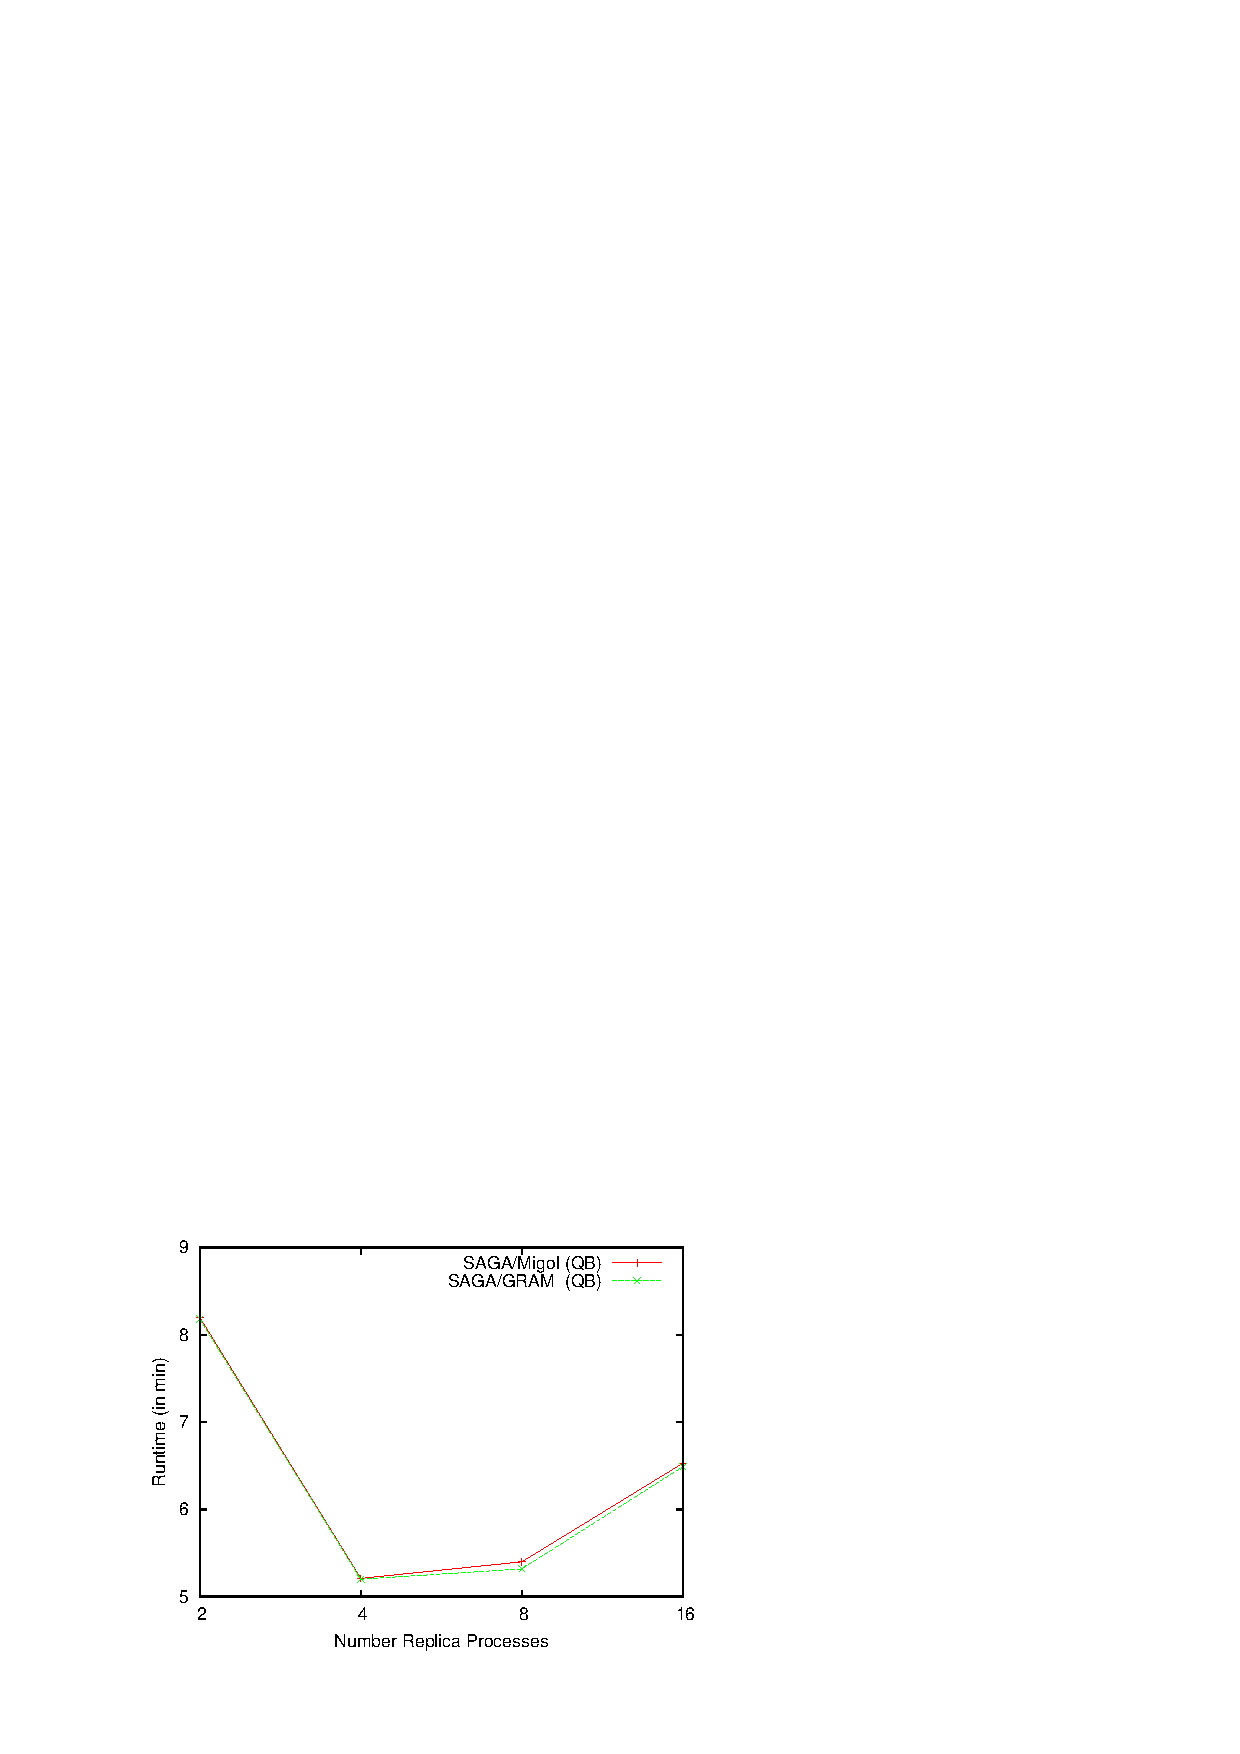
\includegraphics[width=0.5\textwidth]{figures/perf_remd}
    \vspace*{-2.em}
    \caption{\footnotesize REMD runtime shows a
          reduction in time-to-solution for the same
          number of exchanges over multiple
          resources (one system/two systems). 
          Proof-of-concept development indicates that
          the reduction increases with the number of distributed
          resources~\cite{saga_papers}}
    \vspace*{-1em}
    \label{fig:performance_perf_runtime}
\end{wrapfigure}     

First and foremost it is a general purpose framework that can be used
over a wide-range of distributed production environments, such as the
TeraGrid, UK's NGS, DEISA, etc., as opposed to WISDOM~\cite{wisdom},
that is essentially confined to gLITE/EGEE. Secondly, our approach can
scale to use resources of different sizes, as opposed to {\it
  Folding@home}~\cite{folding} which is based upon BOINC, and is thus
inherently limited in the size of physical problems that can be solved
effectively.  Thirdly, our framework is extensible: it can be used
to implement many other application in addition to those based upon RE
simulations~\cite{escience07}. The power to do so arises from simple
design decisions: the use of standard interfaces on the one hand, and
the use of appropriate programmatic and system abstractions that allow
users to do what they can do best (i.e. provide the simulation and
orchestration logic), whilst ensuring that middleware used provides
required services (such as checkpoint management, application
monitoring and recovery) seamlessly and effectively from the
application developers perspective.

As illustrated in Figure~\ref{fig:REMD-Manager-architecture}, the
proposed framework comprises of three components: The task manager,
(\emph{REMD-Manager}), is the end-user program which
encodes the orchestration and replica exchanging logic.  In this
case there is the additional component of a fault-tolerant
infrastructure (Migol~\cite{migol,Luckow:2008xy}) -- that submits, monitors, and if required,
recovers replica simulations.  The last element is the task agent 
(\emph{NAMD-Launcher}), that resides on the High Performance machines
where MD simulations are performed, and is responsible for spawning and
monitoring the MD run. Our RE studies use
NAMD~\cite{Phillips:2005gd}, a highly scalable, parallel MD code, 
to carry out the MD simulation corresponding to each replica
run. It is important to mention that any other MD code could be used
just as simply and effectively.


Figure~\ref{fig:performance_perf_runtime} shows how the
time-to-solution (i.e. wall-clock time) for a certain number of
replica-exchange steps goes down as the number of resources increases.
It is important to note that for the end-user, the complexity of using
one resource is the same as using multiple resources; however, the
gains increase with every added resource (there remain challenges
associated with scheduling the jobs to ensure high-throughput, but
that is not a user-level issue but a system-level one).


\subsubsection*{Example 2: Kalman-Filter-Based Applications:} 

Ensemble Kalman filters (EnKF) are widely used in science and
engineering~\cite{DataAssim, KalmanPaper}. EnKF are recursive filters
that can be used to handle large, noisy data; the data can be the
results and parameters of ensembles of models that are sent through
the Kalman filter to obtain the true state of the data. The variation
in model parameters often has a direct and sizable influence on the
complexity of solving the underlying equations, thus varying the
required runtime of different models (thus the availability of the
results).  Varying parameters sometimes also lead to varying systems
of equations and entirely new scenarios. This obviously increases the
computational size requirements as well as memory requirements.  For
example as a consequence of the variation in size the underlying
matrix might become too large or even effectively doubling the number
of the system of equations, which could more than doubles the memory
required to solve the system of equations.

\begin{wrapfigure}{R}{0.6\textwidth}
 \begin{center}
  \vspace*{-2em}
  \includegraphics*[width=0.6\textwidth]{./figures/3StageKalmanFilter}
  \caption{\footnotesize The irregular execution  of a prototype
   Ensemble Kalman Filter application with
   several stages~\cite{saga_tg08}. 
   Size and granularity of the
   individual models vary, and their runtime is unpredictable.  Thus the resource
   requirements per stage vary dynamically.
   Load-balancing so that all
  models complete as close to each other as possible is the desired
  aim.  There exist many applications that have similar multi-stage,
  global synchronization and heterogeneous ensembles~\cite{dpa-paper}.}
  \vspace*{-2em}
  \label{fig:irregular_execution}
 \end{center}
\end{wrapfigure}     

Hence a mechanism to assign models to available resources based on
their expected time to completion and resource requirement is useful.
Such a mechanism would estimate the time a model will spend in the
queue of a resource, the time it needs to run, and the time required
to migrate the data it requires/produces back and forth, and based on
that attempt to minimize the time required to perform each ``history
matching'' iteration.  In fact, with changing resource simulation
requirements (as is the case with models that find themselves lagging
behind the rest of the model pack), a mechanism which can take
advantage of faster, cheaper or more powerful machines is even more
advantageous ~\cite{escience07}.

We have re-architected a EnKF application, using Cactus for the high
performance aspects, and SAGA for distributed aspects.  Specifically,
Cactus provides the support and features required to implement
adaptivity e.g., checkpoint, restart and migrate thorns. SAGA provides
the ability to implement these features in a specific distributed
environment, for example, move files from location A to location B,
start a job on resource X from resource Y.  Thus the two programming
abstractions that Cactus and SAGA provide are natural complements of
each other.  The result is an application that uses these two
important application-level frameworks and abstractions to create a
power distributed application.

% SAGA provides the capability for the the distributed aspects. SAGA
% provides a high-level programming interface to Grid functionality,
% and thus presents arguably, for the first time ever, the ability to
% develop complete and sophisticated applications using simple Grid
% function calls.  This paper demonstrates the utility of SAGA for
% creating applications that can perform across dynamic and
% heterogeneous infrastructure.

The integration of SAGA and Cactus highlights the advantages of proper
programming abstractions usefulness for developing powerful
distributed applications and novel execution-modes.  Importantly,
although we focus on a prototype of a specific application -- EnKF for
reservoir simulations -- thanks to the architecture and abstractions
used, similar functionality can be trivially incorporated in more
sophisticated and complex applications which have the same application
characteristics~\cite{dpa-paper}.



\subsubsection*{Example 3: First Principle Distributed Applications}


%GridSAT and Network Performance Aware Applications
% GridSAT has been carefully written from ``first principles'' to be a
% Grid program.

We briefly discuss GridSAT~\cite{gridsat03} to provide a {\it classic}
example of a ``first principles'' distributed application written to
achieve scientific results. It incorporates a sophisticated scheduler
that constantly monitors both the progress of the internal algorithm
and forecasts of future batch-queue waiting times, CPU, memory, and
network capacity generated by the Network Weather
Service~\cite{nws-arch,nws-handbook}.  Using these on-line
predictions, the application both proactively and reactively acquires
and releases resources to optimize the parallel search and the
distribution of an internal database.  GridSAT represents a new
generation of Distributed programs not derived from a legacy parallel
code, and is capable of exploiting a heterogeneous and dynamically
changing Grid resource pool.
% The new scientific results it has generated in the form of solutions
% to previously unsolved problems required the use of TeraGrid and ETF
% resources including Datstar at SDSC, all three IA64 DTF machines, and
% Lonestar at TACC in conjunction with cycles harvested from
% workstations.
GridSAT is a realization of cyberinfrastructure's potential and the
science that realizing this potential will make possible. However it
is too complicated to discuss here and we have not actually interfaced
it with SAGA\footnote{GridSAT remains high on our priority list to
  interface and re-architect using SAGA, to both validate SAGA's
  design and stress-test its implementation}, hence we will focus on a
simpler first principle application -- a network performance aware
application~\cite{saga_escience07}, that is able to determine an
optimal resource-based upon dynamical network performance
characteristics and requirements.  This is an applications that is not
amenable to a single, unified programming approach.  The use of SAGA as
a programming abstraction along with a component-based programming
model (such as Cactus) opens up the possibility of creating novel and
interesting e-Science applications.  Although the space of novel first
principle distributed applications has not been explored or scoped, it
would be unfair to dismiss this class of distributed applications; it
is precisely such distributed applications where the whole comes
together to be greater than just the sum of the parts.

% In particular, using SAGA we developed an elementary \I{resource
%   performance} aware application~\cite{saga_escience07} -- which will
% be extended by the Numerical Relativity group as a tool to determine
% the optimal set of resources for their distributed and tightly-coupled
% applications.
% In this work we have deliberately chosen to focus on 
% \jhanote{SAGA-RepEx represents a novel execution mode of otherwise
%   legacy statically distributed applications and finally the others --
%   UCoMS, SCOOP and Numerical Relativity -- represent a medley of
%   workflow style applications, tightly-coupled simulations, static
%   parameter sweeps etc.} 
% It is imperative to note that we are not developing the applications
% per se for the several projects in the third category, but having
% developed the interface and adaptors, we are providing the initial
% support for scientists from those projects to develop applications;
% hence the claim that SAGA is a strategic enabling technology for Grid
% applications.

\subsubsection*{Example 4: Frameworks to support Distributed Application
  Patterns}

% \jhanote{not sure how to use the next couple of paragraphs} The Simple
% API for Grid Applications (SAGA)~\cite{saga-core,saga_web} is a
% high-level programming interface being developed as an approach to
% solve the fundamental challenge in distributed computing: reducing the
% barrier for the development of truly distributed applications. To
% achieve this, it is critical to provide the right abstractions at the
% applications level, to enable applications to be developed independent
% of the specifics of the underlying deployment infrastructure (such as
% middleware distributions, cloud environments, etc.,) and applications,
% once developed, must remain portable and immune to the evolution and
% dynamics of their environments. Additionally, the programming
% interface should cover a broad range of different programming
% paradigms and usage scenarios and therefore, it should not be
% restrictive.

% SAGA had been designed with the fundamental aim of enabling
% compute-intensive applications to utilize distributed environments, by
% providing a high-level, semantically consistent programming
% abstraction and a uniform interface to distinct flavors and versions
% of distributed runtime environments.  The abstractions addressed by
% SAGA are currently file and replica management, job submission and
% control, remote procedure calls, and streaming, are mainly oriented
% towards compute-intensive applications, and being added are
% %Extensions to these abstractions 
% %are being developed to handle
%  service discovery, information management, checkpoint 
% management and application recovery. 
% % These high-level, semantically consistent programming abstractions
% % provide a uniform interface to distinct flavors and versions of
% % distributed runtime environments.

\begin{wrapfigure}{R}{0.6\textwidth}
 \begin{center}
  \vspace*{-2em}
  \includegraphics[width=.55\textwidth]{figures/figure5}
  \caption{\footnotesize Layered ordering of the various components 
    relevant to the project:
    applications such as RepEx, will be
    re-architected to utilize SAGA, or SAGA-based frameworks which support
    reoccurring patterns like AllPairs.  SAGA adaptors interface 
    to the underlying Middleware.}
  \label{fig:overall_scheme}
  \vspace*{-2em}
 \end{center}
\end{wrapfigure}

Effective application development doesn't just require simple
interfaces to allow uniform access to the different functionality
provided by the deployment and runtime environments, as provided by
SAGA. It also requires support for higher level application models and
patterns.  SAGA addresses these challenges by providing a programming
interface that integrates common distributed programming abstractions
while respecting critical application level requirements: simplicity,
stability, portability, uniformity, and support for higher level
programming models and abstractions. Figure~\ref{fig:overall_scheme}
shows the overall application architecture of different classes of
applications built on top of SAGA-enabled, distributed programming
abstractions.

Our recent work has shown that SAGA is not only a programming
interface on the brink of being a OGF technical
recommendation~\cite{saga-core} that conforms to the above
requirements, but that it also provides sufficient abstractions
allowing the creation of frameworks for different application models,
such as MapReduce, All-Pairs, various producer/consumer patterns, and
truly adaptive applications (in terms of their resource and data usage
patterns).  These models all use SAGA at different
levels~\cite{escience_ahm08, gsoc_saga, fuse_web, escience07}.

\I{A MapReduce framework Using SAGA}: MapReduce~\cite{mapreduce} has emerged as a very
successful and popular data-parallel programming model. In the Google
scheme, it is implemented using files, useing their Global File
Systems. However, the question arises of whether MapReduce is a viable
programming model independent of the underlying infrastructure?  What
are the limitations of the data-parallel programming model? To address
these questions, as well as to validate the abstractions that
the SAGA interface supports, we have recently implemented a complete
stand-alone MapReduce framework that does not depend on any specific
infrastructure! We have written adaptors to Hadoop and to BigTable~\cite{hadoop,gbt},
thus providing the ability to use SAGA-based MapReduce framework in
native infrastructure as well.  We are now developing
(re-architecting) applications that have not traditionally been
written using MapReduce, and are understanding their performance and
limitations. Specifically, we are building sequence alignment and
search applications in that framework.  This is an
illustrative example of the kind of empirical testing that is made
possible using SAGA: one can build infrastructure independent
frameworks upon which applications can be developed.

%\begin{wrapfigure}{R}{0.5\textwidth}
% \centering
%\vspace*{-1em}
% \hspace*{-20pt}
%  \includegraphics[width=.45\textwidth]{figures/figure5}
% \caption{\footnotesize Layered ordering of the various components to
%    ...At the very top level, applications such as mpiBLAST, will be
%    re-architected to utilize active storage systems.  Some
%    applications will be built using frameworks that support commonly
%    occurring patterns.  The frameworks in turn will use SAGA which
%    will be extended to provide abstractions for data-intensive
%    scientific applications.  SAGA also provides homogeneous interface
%    to underlying runtime systems as Grids or Clouds. Through the
%    development of appropriate adaptors for SAGA -- such as BigTable
%    and Hadoop, applications can utilize different systems.}
%  \vspace*{-2em}
%  \label{fig:overall_scheme}
%\end{wrapfigure}

\I{All-Pairs Framework for SAGA:} All-Pairs~\cite{all-pairs} is an abstraction for
solving problems that have a combinatoric element; i.e., that require
all elements of a set $A$ to interact with all elements of set $B$.
These characteristics hold for a surprisingly large set of
biological, chemical, and mathematical problems.  The challenge of
applying the All-Pairs model is to efficiently co-locate data and
computation.  This problem space is not easily mappable to MapReduce,
but its implementation actually shows characteristics that are similar
in terms of compute/data co-location requirements, and in terms of
scalability.  We implemented the All-Pairs in SAGA, and use it to
perform multiple alignment~\cite{escience_ahm08}.

\section{Proposed Research and Development Plan}

% \begin{wrapfigure}{R}{0.48\textwidth}
%   \vspace*{-1em}
% %  \includegraphics[width=.48\textwidth]{workpackages_overview}
%   \caption{\label{fig:wps} \small
%   	\B{Architecture overview:} Pictorial representation of the scope 
%   	and distribution of work packages
%   }
%   \vspace*{-1em}
% \end{wrapfigure}

% \begin{figure}[t]
%     \centering
%         \includegraphics[width=0.45\textwidth]{saga-taskfarming}
%         \caption{\footnotesize \bf Fault-Tolerant MD Simulations: The
%           REMD-Manager orchestrates a set of distributed replica
%           processes using the SAGA API. All processes synchronize
%           important metadata with the Migol infrastructure. Migol then
%           actively monitors all processes and ensures that, even in
%           the presence of failures, all task are eventually
%           completed.\up}
%     \label{fig:saga-taskfarming}
% \end{figure} 


% The goals for research and development of the two teams participating
% in this proposal -- the SAGA team and the GridSAT team -- are
% exceptionally complementary.  On one hand, GridSAT can be enhanced
% with the help of SAGA, resulting in a version that is more portable,
% extensible, and standards based than the current specialized
% implementation.  On the other hand, GridSAT will serve as a test case
% for verification, implementation and validation of extensions to SAGA
% and for stress testing its performance.

% for automated and secure wide-scale deployment across major Grid
% sites, data management for remote file access and inter-process
% communication facilities for instance for message exchange among
% GridSAT nodes.

% Some components of SAGA can be leveraged by our applications
% immediately, simply by using the existing LSU C++ SAGA
% implementation~\cite{saga_web}, for example, job and session
% management, data management for remote file access.  The SAGA team
% will specify extensions to the API required to support additional
% features required by our applications (in synchronization with other
% use cases and the SAGA community) and develop them as part of the
% collaboration.  This includes the information services package for
% service and resource discovery allowing the applications to
% dynamically leverage available resources, a new SAGA package for
% application level checkpointing, and the specification of SAGA
% language bindings accommodating all of this projects applications.
% Figure~\ref{fig:wps} highlights the different work packages, their
% relationship, and the distribution of work between the two teams. A
% timeline of the planned work is shown in Figure~\ref{fig:gantt}, and
% the planned milestones and deliverables are described in
% Table~\ref{tab:wplist}.
 
%\input{workpack-table}

% \B{WP-1 - SAGA-GridSAT:} GridSAT~\cite{gridsat03} is
% arguably the first application written specifically for distributed
% environments; it is the classic prototype of a Grid application.
% Having tested the limits of what a Grid application can do without
% regard for extensibility, maintainability, and packaging for re-use,
% we are now eager to replace the brittle, customized distributed
% computation platform .... % of GridSAT with SAGA and to make the code
% available to the wider SAT community.

% Our re-implementation of GridSAT will retain some components intact:
% namely, the original zChaff~\cite{chaff} SAT solver and our parallelizing
% modifications~\cite{gridsat-sc03}, as well as the core logic of the
% \emph{scheduler}.  
% .... Much of the Grid-related code, however, will be
% reimplemented using SAGA and modularized in the form of a \emph{manager}.
% Concretely, we will perform the following tasks. 

% i) We will replace the ad-hoc \B{job submission} scripts and hard
% coded SSH invocations with SAGA's job management and session
% management frameworks, relying on ``security tokens'' for consistent
% access to computational resources available through Globus.
% ii)~Instead of staging the SAT problem input file (containing an
% encoding of clauses) to computational nodes manually, we will use
% SAGA's \B{data management} for transparent replication of file data
% upon access to it by client processes. We will use the SAGA API for
% application level checkpointing to implement the required
% checkpointing functions. iii)~Interprocess communication, currently
% done over a custom messaging library using the socket interface, will
% utilize SAGA's \B{streams} API instead, for overall consistency.  Once
% a NAT/firewall proxy is developed with the help of SAGA, it will be
% incorporated into the GridSAT communication model. iv)~Our \B{resource
%   management} interfaces, currently configured to collect information
% from NWS and MDS, will utilize SAGA's information services API for
% uniform access to information about available nodes and predictions of
% CPU load, bandwidth, latency, and batch queue wait times.  The two
% teams will work together on adding batch queue prediction
% service~\cite{bqp} into the information services package of SAGA.
% v)~\B{RPC-style} invocation is a natural mode of interaction between a
% client and the GridSAT master (i.e.\ clients invoke a procedure on the
% master either periodically, as in the case of ``heartbeats,'' or when
% an important event occurs, such as job completion or timeout).  We
% will therefore use the corresponding SAGA GridRPC API simplifying
% GridSAT code and making this functionality available to other
% applications. 

\B{WP-1 - The SAGA engine - the central component:}
The Core SAGA Library (referred to as SAGA Engine)  has been
under development since Fall 2005 (supported by internal CCT funds).
Until now, the engine has matured significantly but it still needs 
to move out of research prototype status to production quality
and to being ready for deployment on a wide range of platforms. This 
workpackage will focus on the development of the SAGA engine and the SAGA 
packages based on use cases gathered from the development of
SAGA applications. At the same time this application development has revealed a couple of
deficies in the current SAGA specification and implementation. For this 
reason we propose to extend the SAGA engine with new functionality, 
while fixing the problems encountered so far. The following list gives a
short overview about planned activities in this regard:

\begin{shortlist}
	\item Provide the possibility for adaptors to take advantage of bulk-oriented
	      optimizations
	\item Improve asynchronous operation support by optimizing the internal
	      structure of the engine and the introduction of thread pools 
	\item Add new API packages to the SAGA distribution as new specification
	      extensions get developed and adopted
	\item Solve semantic and implementation problems related to asynchronous
	      late adaptor binding and merging of results provided by several adaptors
	\item Add support for task dependencies, a major precondition for the integration
	      of SAGA with workflow-based systems
	\item Improve ease of deployment and cross platform capabilities over a
	      range of different target platforms and middleware distributions
\end{shortlist}

The \B{measure of success} for this workpackage is twofold.  First, the
improved code quality, standard adherence, and cross platform
capabilities should foster the adoption of SAGA on multiple middleware
backends.  Second, improved engine capabilities will support both the
specification and implementation of higher level programming
abstractions -- we expect to see standardization activities on that
level, mostly focused on data and work flow centric use cases, and
also expect to see implementation activities utilizing both the
improved bulk optimization capabilities, and the improved late binding
capabilities.\\[-0.5em]


\B{WP-2 - Specification and Verification of SAGA Extensions:}
\amnote{too long?  Is a combination of former WPs 2 and 3...}
This work-package will focus on two areas: i) specification of
SAGA API extensions as required by the set of applications
(information services, application level checkpointing, and
workflow), and ii) language bindings of the extensions, and
verification thereof.

\I{Specification of SAGA extensions:}  Our previous work (see
Section~\ref{sec:previous_work}), and collaborations with
external groups, for example in a Google Summer-of-Code project
with the University of Western England, Bristol, exposed
a number of high priority areas for future extensions to the
SAGA API scope\footnote{Note that the SAGA API scope as defined
at the moment is limited on purpose, but SAGA is designed to be
extensible on that level, and extending SAGA's API scope that
way is a declared goal of the SAGA standardization group in
OGF}.  Among these extensions are (1) interfaces to information
services, for storing application chunks level information
persistently; (2) interfaces to checkpoint and recovery
facilities, and to checkpoint management functionality; and (3)
interfaces to programmatically express and execute workflows, or
data flows.

\I{Information Service API:} The specification of the
information services packages will have to ensure that the
interface has the ability i) to manage arbitrarily structured
data, ii) the identification of data items via an hierarchical
name space should be possible, iii) have the ability to search
this namespace and the data items, iv) allow data persistency,
and v) should allow simple management and navigation of
collections of data item. The main challenge here is indeed that
neither syntax nor semantics of the data items to be stored are
well defined or standardized, and vary widely over the known use
cases.  It is proven to be difficult to remain agnostic to data
syntax and semantics, and still provide a scalable and
\I{simple} solution.  
% Respecting all these constraints will be a challenge.

\I{Checkpoint and Recovery:} The package for application level
checkpointing and recovery will not only provide a uniform
interface to different application and system level
checkpointing mechanisms, but it will provide additional means
of i) associating metadata with specific checkpoint files and
ii) managing (i.e. store, find and retrieve) checkpoint files.

\I{Workflow support:} The SAGA core API supports the notion of tasks
as asynchronous operations, which are absolutely essential for
efficient distributed applications.  As a simple extension to that, we
plan to introduce conditional task dependencies, which will allow us
to express work flows as DAG of SAGA tasks.  Related, we plan to
support data driven work flows, aka data flows, where application
defined data item are exchanged between successive tasks.  Finally, we
plan to extend the job management facilities to allow the submission
of abstract workflow and dataflow descriptions, to the respective
enacting middleware. We will be very careful to not repeat or reinvent
many of the advances made in the workflow technology; we will be sure
to adapt to and use existing software~\cite{saga_condor_talk} and
tools, while still being able to support the programmatic construction
of simple workflows using SAGA.

We will ensure that i) the new packages cover application needs, ii)
the specified new SAGA packages are consistent with the existing SAGA
API -- with both the packages as well as different calls of the API,
iii) the new packages meet the portability criteria established by the
existing SAGA code base, iv) the new packages interoperate properly
with the existing code base and with each other and v) are
semantically consistent.  Verification of the developed specification
goes hand in hand with the reference implementation of the SAGA
extensions and corresponding tests done as part of WP-4. 

Along with the definition and implementation of the SAGA API packages,
we will also provide the respective middleware bindings, based on
Globus Toolkit Version~4, where appropriate.  Specifically, we will
implement a set of dynamically loadable adaptors to connect to
NWS~\cite{nws} and WS-MDS~\cite{globus_web} for the information
services package, and a special adaptor implementing the required
functionality for the application level checkpointing package.  The
adaptor behavior will have to be validated with the existing C++
implementation and middleware distribution.  Note that the workflow
related implementation work is tightly coupled to the engine
development tasks listed in WP-1, and will only require limited
implementation work on adaptor level.

The \B{measure of success} for this work package is (a) that both
extension packages enter the OGF standardization process, and (b) that
application are using these extensions, and prove the portability and
scalability of the implementations.\\[-0.5em]  

\B{WP-3 - SAGA-based application frameworks:} The ultimate goal of
SAGA to provide simple effective means to use distributed CI for
application developers, implies that the SAGA does not stop at the
abstraction of low level Grid functionality, such as job management,
data access, or communication (that is the level of WP-2), but goes
further up the abstraction chain and provide support for programming
patterns.  We expect that higher-level abstractions, such as
collective operations, master-worker paradigms, MapReduce and
AllPairs, will play an equally important role in supporting novel
distributed applications.  In particular the rather young data
centered distributed data frameworks, such as MapReduce and Hadoop,
show great potential.

In this work package, we intent to implement several of these
frameworks, on top of the existing SAGA implementations:

\begin{shortlist}
	\item master-worker framework: a persistent manager of large
  collections of loosely coupled tasks, with failure recovery and
  opportunistic scheduling;
  \item support for other commonly occuring usage modes, such as
  exchange and migration
	\item long-lasting application manager: a container for very long
  lasting applications (order of weeks), with the ability to 
  checkpoint/restart, and to migrate applications;
  \item Research toward other, novel distributed programming models
\end{shortlist}
\up

% \jhanote{Mention also how day-in-the-life can be used as a
%   checkpointing and migrating frameowrk}.

This workpackage is expected to deliver implementations which are
useful well beyond the set of applications considered in this project.
Due to (a) the generic nature of the targeted frameworks, (b) their
portability due to their SAGA foundations, and (c) their ease of use,
we expect rapid uptake, if delivered timely.  Other implementations of
these frameworks are of course already available, but show either are
only available in a single programming language (whereas SAGA has
multiple language bindings), or are tightly coupled to a specific
middleware platform (whereas SAGA decouples applications from the
backends).

It remains a challenging technical task to provide the above listed
frameworks as high-performaning and scalable implementations, despite
the middleware decoupling.  The metric of success for this workpackage
is to demonstrate one application per framework, on two different
middlewares, with performance and scalability characteristics in the
same order as middleware bound implementations, where these are
available.\\[-0.5em]


% \begin{figure}[!]
% \up\up
% %  \includegraphics[width=1.0\textwidth]{workpackages_GANTT}
%   \caption{\label{fig:gantt} \small Timeline of the planned work.
% }
% \end{figure}

% Based upon our experience of specifiying the interface upto now, we
% realize the challenges that the theoretical derivation and
% specification of abstractions poses.  (MPI specification process is an
% interesting guide). These complexity and challenges will be magnified
% as we try to come up with programming interfaces and abstractions for
% more complicated functionality as embodied by information services --
% which although complicated, is critical for dynamic, Grid-aware
% applications.

%To achieve this, we will implement a set of dynamically loadable
%adaptors to leverage different services provided by the Globus Toolkit
%version 4 Web Services~\cite{globus_web}, namely WS-GRAM for job
%submission and monitoring, RFT for reliable file transfer,
%Ninf-G~\cite{ninf-g} for executing remote procedure calls, and
%NWS~\cite{nws} and WS-MDS for information services. The proposed
%adaptor set will cover the complete middleware functionality needed by
%GridSAT and will thus render GridSAT deployable on any GT4 Grid.  
%\B{'C' language bindings for SAGA:} 

% The C++ SAGA implementation at LSU/VU has the following design
% principles: i) As much logic and functionality as possible has been
% built into the SAGA library core, providing all the needed common
% functionality. This enables us to extend our SAGA implementation with
% minimal effort.  On the other hand, the library is designed to be easy
% to build, use, and deploy. ii) Another major design objective is to
% maximally decouple the different components of the developed library,
% so as to provide as much \I{flexibility}, \I{adaptability} and
% \I{modularity} as possible.  iii) As the SAGA implementation is
% expected to be used on different platforms and operating systems we
% strive for maximal implementation \I{portability}.

% In order to also leverage these design objectives for the SAGA C
% implementation, and to enable significant code reuse (for the SAGA
% engine and all available SAGA adaptors), we will develop the 'C'
% language bindings as a thin layer on top of our C++ implementation.
% This language binding will simplify the integration of the GridSAT
% (partially written in 'C') with SAGA.  Additionally the availability
% of C bindings will enable the uptake of SAGA by an entire class of
% applications written in C.


% This adaptor set taken together with the already existing SAGA
% adaptors will cover the complete middleware functionality needed by
% the application suite and will thus render these applications
% deployable on any GT4 Grid.

% The bulk of the remainder of WP-3 will be devoted to supporting GridSAT
% integration efforts at all levels -- from syntax tweaks of the
% interface, all the way down to adaptor installation and debugging.
% Qualitatively similar support will be required for the ``other
% applications'' by groups external to this project that have indicated
% a need and desire to integrate SAGA with their applications or develop
% tools using SAGA.  A final part of the application integration
% component of this WP involves writing a simple ``master'' application
% (SAGA-RepEx) for biomolecular simulations.  With the interface
% specified and validated from GridSAT, as well as the required adaptors
% implemented and deployed, this will be an easy and quick validation of
% the power that a high-level programmatic approach to marshaling
% resources and controlling distributed functionality provides.

\B{WP-4 - Integrating SAGA with Applications:} Our target applications
are listed in Table~\ref{appsuite}.  It is worth mentioning that these
applications have been carefully chosen and cover almost the entire
spectrum of distributed application classes~\cite{dpa-paper}. The PI's
group~\footnote{Jha is the Interim lead of the Material World focus
  area at the CCT, with funded projects in the Biological Sciences,
  Physical Sciences, theoretical computer science and infrastructure
  development projects} overlaps computational science and
cyberinfrastructure development and is thus uniquely positioned to
provide prototypes from each Appliation Class.  WP-4 is unique in that
it will enable development and deployment efforts in other work items
to actually deliver scientific results.  This WP is not concerned with
the scientific results themselves, but in enabling the real world
applications to utilize production infrastructure towards that
end. Our efforts will not remain confined to the set of applications
outline in Table~\ref{appsuite}; it would be a direct validation of
our efforts if our solutions were used outside of our own project and
group.

\begin{table}[h]
\begin{center}
  \begin{tabular}{|l|l|}
    \hline

    \B{Application Area}                            & 
    \B{Application/Project}                         \\\hline

    Pleasingly Distributed Tasks                    &  
    Monte Carlo Simulations of Viral Propagation    \\\hline

    Loosely Coupled Homogenous Tasks                &  
    Replica Exchange Molecular Dynamics of Proteins \\\hline

    Tightly Coupled Homogenous Tasks                &  
    Heme Lattice-Boltzmann Fluid dynamics           \\\hline

    Loosely Coupled Heterogeneous Tasks              &  
    Kalman-Filter Fluid Dynamics                    \\\hline

  % Dynamic Data-Driven Applications                & 
  % \jhanote{think hard}                            \\\hline

    First Principle Distributed Applications        & 
    Network Performance Aware Adaptive Application  \\\hline

    Data-Parallel Applications                      & 
    MapReduce-Based Motif Distributed search        \\\hline

\end{tabular} 
\caption{\small The application classes and specific application
  examples which cover the primary categories~\cite{dpa-paper} of
  Distributed Applications. WP-4 will implement and/or 
  re-architect these specific applications from the given 
  application classes using SAGA.
  % These examples are not just excercises
  % in software engineering, but of geniuine scientific interest to the
  % proposing group and will serve as important representative prototypes for a 
  % large fraction of scientific applications on the TeraGrid.
}\label{appsuite}
  \vspace*{-1em} 
\end{center}
\end{table}
\upp

% Our target applications are listed in Table~\ref{appsuite}.  The
% respective application groups are not part of the project, in terms of
% funding, on purpose: we consider it a far greater challenge, but also
% a far greater success, to find our solutions to be used \I{outside} of
% our own project and working group.  As only the SAGA side is funded in
% this work package, we cannot rely on the durable commitment of all of
% these application groups for the duration of the project.  The
% \B{measure of success} for this work package is that two or more of
% the applications listed are interfaced or re-architected (as needed)
% using SAGA for deployment on production distributed environments.\\[-0.5em] 



\B{WP-5 - Deployment on Production Infrastructure and Interoperation:}

\I{Deployment:} Successful deployment of SAGA on the TeraGrid has
several critical advantages and is one of our key goals: first, as a
powerful computational platform, the TeraGrid is ideal for attempting
scientific problems of unprecedented size and complexity.  Second, as
an extensive system of distributed services and resources, TeraGrid
will be a challenging environment for evaluating and stress-testing
SAGA.  We expect problems in design and in implementation to reveal
themselves as we attempt to scale the applications from WP-4 onto the
TeraGrid, both in terms of size and heterogeneity.  Finally, as a
popular production computing environment, TeraGrid will ensure that
upon success of many other TeraGrid applications will be able to
utilize SAGA with minimal effort. In all of this, the support of the
TeraGrid software integration team will be critical; we are very
fortunate to have been assured of it \jhanote{(Skow - Letter of
  Support)}.

Additionally the planned deployment of SAGA on the TeraGrid lays the
grounds for other applications to leverage application level
functionality. To reach beyond TeraGrid, we plan to simplify the
creation of binary SAGA distributions, in a range of formats, such as
tgz, rpm, and deb.



% eg \firstprincipleapplication\ has been deployed on a few LONI sites
% before, but the inflexible architecture of the current implementation
% prevented us from a large-scale long-running deployment. 
% \jhanote{Andre, Hartmut, Ole: I'd like you to outline the challenges
%   of deployment, what are the areas of improvement that we need to
%   address and any other suggestions that you have. We can even
%   introduce the request for a re-architected saga-lite along the lines
%   that we discussed in the call today, just that we can't call it
%   saga-lite}

\I{Grid interoperability:} Establishing Grid interoperability is
non-trivial, but critical if scientific applications want to
use their local regional infrastructure but also want to
progress toward larger and more distributed resources.
With the demonstrated reduction in time-to-solution for
Replica-Exchange as an exemplar application, it is self-evident
that interoperability is not just of academic interest, but of
practical importance.

It is critical to contrast our approach to interoperability with
the other efforts such as those of the GIN-CG group: many if not
most efforts are based upon establishing interoperability at the
service and feature level. In contrast SAGA believes in {\bf
Application Level Interoperability}, and in ~\cite{saga_gin07}, we sketch how the three main components
of the SAGA landscape -- interface specification, core engine,
and middleware-specific adaptors -- facilitate interoperability
across Grids.  SAGA thus provides a promising path for the
rapidly growing number of applications~\cite{clade06,
cc07_spice} that require portability across a range of
distributed environments, i.e., the ability to inter-operate
across a range of federated Grids, for instance, regional infrastructure
such as LONI and national-level infrastructure such as the
TeraGrid, as well as peer Grids such as LONI and SURAgrid.  Our
effort in this workpackage will be to establish application
level interoperability using SAGA, for the suite of applications
discussed in Table~\ref{appsuite}.  This will provide further
testimony to the claim that SAGA represents a simple yet
strategic technology.\\[-0.5em]



\B{WP-6 - Outreach, Education, Support and Dissemination:}

The PI's group is uniquely placed to lead Education, Support and
Dissemination activities: the group has been involved and leaders at
every stage of the SAGA pipeline, all the way from the SAGA
specification process at the OGF, to providing the first
implementation (C++) and language bindings; critically being early
developers of applications and prototypes as well as being involved
in the deployment of applications using SAGA.  Thus we are well placed
to develop a SAGA users manual and a tutorial based upon our
experiences. OGF is a great place to begin our outreach activities --
especially given their strong emphasis on enterprise applications, and
on teaching and educational activities.  We are in discussions with
Malcolm Atkinson, who leads the education and training activities of
the OGF. We will also reach out to communities typically not attending
OGF.  But through all of this, the fundamental work will be that of
writing i) easy to read SAGA manual/users guide, ii) tutorials on
SAGA and how to adapt applications to use SAGA.  These activities will
be a critical step in ensuring that the benefits of SAGA reach new
application and user communities.  Feedback from hands-on sessions
(the CCT has extensive experience in hosting such hands-on sessions)
and user feedback will help to improve and debug the implementations.
Our EOT efforts will build upon preliminary work that has already
begun~\cite{eot_url1, eot_url2, eot_url3}; for example we delivered a
half-day tutorial at Grid2007 (Austin), a half day tutorial at the
International Summer School on Grid Computing (Hungary, 2008) and have
agreed to deliver {\bf pro-bono} a 2 day training program for the UK's
National e-Science Centre and National Grid Service (most likely in
January 2009; final details pending, but will be made available at
http://www.nesc.ac.uk/training/events/index.cfm)

\section{Related Work}
\label{subsubsection:other_saga_work}

% \B{Other SAGA Implementation:} The DEISA project has developed a
% partial SAGA Java implementation~\cite{deisa_saga} that binds to the
% DEISA job submission and data management services.  The NAREGI project
% is developing another partial SAGA Java implementation, focusing on
% the SAGA job submission package, that binds to the NAREGI middleware
% stack.  There is also work within the EGEE project.  These are often
% partial implementation of SAGA (specific packages) for their own
% middleware stack (e.g., to achieve mostly uniform job submission) and
% often are just SAGA wrappers to specific services.  Whereas this is
% testimony to the allure of standards and the willingness to conform to
% standards -- especially for Grid environments, simple software
% engineering activity as represented by these partial implementations
% does not involve \B{the coupled process of interface specification,
%   validation, applications implementation and deployment} and does not
% contribute to the specification and standardization process. Our group
% has been at the vanguard of the specification, implementation and
% application development and is uniquely placed to drive this effort.

%% \jhanote{need to reiterate that we can implement programming modes
%%  in a infrastructure independent way; tie this better to the DPA 
%%  part}
%\B{Distributed Programming Abstractions:} 

\B{Research Theme on Distributed Programming Abstractions:}~\label{dpa}
PI Jha and SI Katz have been leading a two year long UK e-Science
Institute theme on Distributed Programming
Abstractions~\cite{dpa-paper,dpa-wiki}.  (Jha also serves as the PI of
the theme.) At a general level the theme aims to understand the main
barriers to the widespread adoption of distributed applications, and
how scientific applications - both compute-intensive and
data-intensive - should be programmed such that they are easily able
to utilize a distributed infrastructure? More specifically, the theme
is trying to understand the landscape of distributed applications --
different types, primary characteristics, and the development and
deployment tools for each type.  Thanks to many years of experience
and research, it is relatively easy to determine which algorithms and
data-structures should be used such that application codes scale well
across a single platform, but the analogous ideas are not well
developed for distributed computing.  For example, what are the
distributed analogs of ``Parallel Dwarfs'' (recurring programming
patterns) as laid out in The Landscape of Parallel Computing
Research~\cite{landscape}?

In its first year, the theme has systematically analyzed a range of
real distributed scientific applications, defined a set of ``vectors''
used to characterize these applications (into essentially
non-overlapping classes), identified a series of patterns --
programmatic, deployment and usage modes -- associated with these
applications and begun the process of identifying suitable
abstractions to support these commonly occurring patterns.  In the
near future, the theme leaders will be providing a gap analysis
between existing tools and programming methods and the patterns
identified. We are also finalizing negotiations with Wiley to publish
a book on Abstractions for Distributed Systems.  The application
patterns that we will be developed as part of this proposal will be
informed by theoretical studies that the theme carries out; in turn
input gained from implementing these using SAGA will be fed to the
theme.  A unique feature of this theme is the strong coupling between
distributed programming models, techniques and abstraction on the one
hand and real applications on the other to first explore programming
models and abstractions in detail and then apply them to specific
application classes and domain.  One of the explicit aims of this
theme is to help understand how SAGA can be extended to new functional
areas, as well as improve upon existing areas, to support distributed
programming. The theme will provide important but independent
intellectual support for this proposal and help inform the future
evolution of SAGA.

\B{Java implementations of SAGA: } There has been a flattering if not
bewildering level of uptake of our SAGA effort in Europe.  Several
groups have taken the SAGA specification -- which we have led and
contributed to -- and have developed independent implementations of
the specification. We mention in passing the JSAGA project~\cite{jsaga}
as one of the exemplars (noteworthy if nothing else for the fact that it
is supported by several companies, such as British Telecom). However,
we focus on DEISA, which by many accounts is the project most similar
to the TeraGrid.  In particular, we identify DESHL~\cite{deshl_url}
(colloquially referred to as the DEISA shell, but rigorously DEISA
Services for Heterogeneous management Layer), which uses the SAGA API
to provide a uniform interface to launch and manage jobs on all DEISA
resources. These are essentially simple wrapper scripts around the
basic SAGA API calls. The DEISA project has recently gone a step
further and have developed advanced ``submission scripts'' for
scientific simulations~\cite{ssss_deisa} on DEISA; these are simple
``workflow'' and ``job orchestration'' scripts developed and made
available to the entire DEISA user community. In other words, these
are very powerful system-level ``applications'' that arise from having
basic SAGA functionality supported on production level infrastructure;
these scripts in turn then bring out the power of the ``D''
(Distributed) in DEISA, while ironically abstracting the
distributedness via SAGA.  The power and the subtleties of
abstractions!

\jhanote{Andre, if you think it makes sense, please work in something
  along the lines of the submission scripts for DEISA into one of the
  workpages?}

% \href{http://deisa-jra7.forge.nesc.ac.uk/}{http://deisa-jra7.forge.nesc.ac.uk/}% but that make abstract the ``D'' in DEISA but provide the power of the
% ``D'' (Distributed) The power of abstraction!
% http://www.fz-juelich.de/nic-series/volume38/pringle.pdf

\B{Computer Science Research: } Interestingly, there are groups in
Europe that have started utilizing advances made in SAGA, especially
our C++ development and middleware adapter set for further research in
computer science. A particular noteworthy example is the XtreemOS
project~\cite{xtreemos} which aims to develop a a Linux-based operating systems to support
``virtual organizations'' in the next generation of Grids.
\jhanote{Andre: Do you have ideas/links on how SAGA is being used by
  XtreemOS? I have slides, but no write-up}

\section{Intellectual Merit and Broader Impact}

\up\up

An indicator of SAGA's strategic importance is also a measure of
SAGA's success, namely the number of new Grid applications that are
developed, the kind of novel usage scenarios, as well as the ease and
wider usage of existing applications that SAGA enables.  An important
aspect of the proposed work and further confirmation of the {\it
  strategic} role of SAGA is our aim of enabling the development of a
significant number of diverse applications -- varied in discipline,
type (data versus compute) and Grid functions involved.  Table
~\ref{saga-takeover-world} provides a reduced overview of some target
applications and application areas.

\begin{table}
\begin{center}
  \begin{tabular}{|l|l||l|l|}
     \hline \B{Area} & \B{Application/Project}  &  \B{Areas}  & \B{Application/Project} \\
      \hline Astronomy  & Montage (JPL/NASA)
      &  Coastal Modeling &  UCoMS (Allen) \\
      \hline Biological Sciences & Replica Exchange 
      & Lattice Fluid Dyn & HemeLB  (London/Tufts) \\
      \hline Computer Science & CoreGrid (Rosa Badia) 
      & Numerical Relativity & Cactus (Schnetter) \\
      \hline Visualization & DIVA (LBNL)
      & Interactive Viz. & LONI (Hutanu) \\
      \hline Bioinformatics &  Protein Pattern Scanning 
        & Comp. Biology & Hybrid MC-MD (LBNL) \\

      \hline 
\end{tabular} 
\caption{\small Some of the science areas and applications that have
  either submitted use cases in document GFD.70~\cite{saga-uc} or are
  working towards using SAGA for their
  applications/projects}\label{saga-takeover-world}
  \vspace*{-1em}
\end{center}
\end{table}


To summarize, the proposed work has the potential to significantly
advance research and education capabilities in multiple areas of
science and engineering because:
\begin{shortlist}
\item The SAGA effort has received input from a broad range and number
  of applications; its scope and design is based upon analysis from
  this broad applications community~\cite{saga-req}.
\item Engagement with TeraGrid and the wider International Community.
  SAGA's deployment on the TeraGrid (and elsewhere) will enable
  significant numbers and new usage modes of applications.
\item A unique feature of our work plan is its dual strategy: a
  fast-track integration of applications with SAGA that
  will drive the deployment on the TeraGrid, coupled with a deep-track
  exploration of the abstraction, extension and validation of the
  specification.  There is strong bi-directional feedback between Grid
  application design and programming and the related specification and
  implementation work.
\item A large number of projects have expressed interest in using
  SAGA -- formally and informally. It is not possible to directly
  support all the integration efforts, hence the need to develop
  effective and comprehensive manuals and tutorials. These will then
  provide positive feedback so as to increase the attractiveness of
  SAGA to other application communities. Additionally, the SAGA effort
  has strong support in the OGF which has its own very active and
  effective dissemination and outreach activities -- spanning the
  global academic community, enterprises and the humanities and
  social-sciences % (HASS)
  domains.
\end{shortlist}

The work in this proposal will be done at LSU, in an EPSCoR state.  We
are also working on an statewide NSF EPSCoR project generally referred
to as Cybertools~\cite{cybertools_url}, which is aimed at advancing
both tools/services and applications at the same time by using each to
drive developments in the other.  This work will fit directly into the
tools/services part of Cybertools.  Cybertools also has a set of
education activities to which this work will be added.  These include
summer boot camps for high school students, including predominately
minority schools, and summer research projects for undergraduates,
where we successfully strive to find students from underrepresented
groups.  Additionally, PI Jha and SI Katz (with LSU CS Prof. Gabrielle
Allen) are planning a graduate course in Abstractions for
Distributed Systems, where lessons from this project will be taught.

LSU operates the LONI network and distributed high performance
computing (HPC) resources for the state of Louisiana.  In this role,
we provide statewide training to potential HPC and distributed
computing users.  We will include the results of this work in our
training workshops.  LSU is also a driving member of SURAgrid, so this
work will be pushed out across the SURA region, which has been shown
to have a relatively low level of HPC and distributed computing
knowledge and usage compared with the rest of the United States.  LONI
(as led by LSU) is also a Resource Provider (RP) partner in the
TeraGrid, which give us the opportunity to push the results of this
work to other national computing centers and their national audience.

In the remainder of this section, we try and address potential
concerns over the broader relevance of our work to the current state
of cyberinfrastructure.  We conclude this section on Broader Impact by
explicitly addressing a couple of issues that were raised in our
earlier STCI submission.

The SAGA landscape provides a fertile ground for significant training
and research opportunities for both undergraduate and graduate
students.  Chris and Michael Miceli\footnote{see people under ``The
  Team'' at http://saga.cct.lsu.edu} -- computer science
undergraduates at LSU, have been voluntarily working on the SAGA
project as part of their Chancellor's aid requirement. Michael was the
recipient of the Google Summer of Code assistantship during which he
has made impressive progress towards implementing the MapReduce
framework using SAGA and deploying over LONI.  In a testimony to his
efforts, work based upon his summer project funded by Google has been
short listed for publication~\cite{escience_ahm08} in the Philosophical
Transactions of the Royal Society A (London) -- the world's oldest
scientific journal (started by Isaac Newton).  The Miceli brothers are
continuing their involvement with the SAGA project through Fall 2008
and spring 2009 by enrolling in CSC3999 (independent study) under PI
Jha, where they will continue to work on application frameworks for
distributed systems. This is further proof that SAGA provides
comprehensive end-to-end training in Cyberinfrastructure for
undergraduates and thus providing them with an ideal launching pad for a
future career in either academia or industry.
\amnote{Newton is irrelevant.  Here I mean :-)}

% \jhanote{We need to add something about Undergraduate research (just
%   reviewed panel summary. We talk about Miceli's -- test
%   infrastructure, Google Summer of Code, CSC3999, publication for UK
%   eScience Conference and I talk about Ashley}

\paragraph*{SAGA is Not a Middleware} 

For placing this project proposal, it is crucial to understand that
SAGA is not a middleware.  In fact, SAGA does not, in itself, provide
any capabilities of its own, but rather abstracts capabilities
provided by typical Grid middleware systems, in a simple and coherent
manner.


% \paragraph*{Is SAGA Itself Simple Enough? } We (the standards
% community) have designed the Simple API for Grid Applications to be
% simple for \I{application developers} to use and more portable than
% using the direct middleware API's.  But this goal almost necessarily
% implies that the SAGA implementation itself will not be simple;
% Ref.~\cite{saga-c++-engine, saga_gin07} document the challenges
% encountered in implementing SAGA with the often divergent and almost
% incompatible requirements.  The SAGA library core has much of the
% logic and functionality built into it as possible; distributed
% computing environments are complex systems normally requiring
% complex software and the SAGA library core attempts to shield the
% application developer from this complexity by implementing a lot of
% the needed common functionality and by exposing it via simple and
% standardized interfaces.  \jhanote{Reduce next two sections by a
%   bit}

\B{SAGA's User Base is Currently Narrow:} Even though, SAGA is both a
new approach (standardized API for distributed applications) and new
technology, several groups have started to develop specification
conformant implementations.  For this reason the actual {\em user}
base for SAGA is still narrow, but the base stemming from the
standards community is wide.  Before scientific application developers
will commit to the use of SAGA we need to establish and demonstrate
the proof-of-principle.  The suite of applications in Table~\ref{appsuite} are
the first steps in that direction.  Application developers are
unlikely to commit to using an unvalidated and undocumented technology
wholesale, however broad the initial interest and compelling the
technical requirement.  Documenting and demonstrating scientific
applications were ``before SAGA was used'' and ``using SAGA'' will
provide compelling reasons for application developers to commit to
SAGA.  

% The reason SAGA has emerged so quickly as a standard (even with
% a relatively narrow user base) is that it is one of the only
% application level technologies that takes as a mandate both
% application programmability {\em and} the various modalities grid
% applications need to adopt to use federated, distributed resources.
% SAGA provides the right set of generic functionality on the right
% level of abstraction~\cite{saga_escience07}, 
%  At the same time, it has already
% been taken up by the Grid standards community (Version 1.0 of the SAGA
% specification~\cite{saga-core} has been submitted to the OGF editorial
% pipeline and is currently under review) and 
\jhanote{Need to modify: We believe that by demonstrating ``a Grid
  application before SAGA was used'' and ``a Grid application using
  SAGA'', where by in the former case, an application is large,
  difficult to port, extend and deploy but once integrated with SAGA,
  the application is simple, portable, extensible and easily
  deployable, we will have provided a compelling case for SAGA.}

Although, the exact interval can be debated, there was a significant
lag between the MPI specification and a major uptake of the
specification, with several rigorously validated and crafted exemplars
in between.  But as alluded to, the ``chicken-and-egg'' analogy is
applicable for the current state of distributed applications too,
hence we need to establish and demonstrate the proof-of-principle
before scientific application developers will commit to the use of
SAGA.  Our plea is that in conjunction with the other work
items that we propose, WP-4 will provide precisely such a set of
compelling exemplars.
Additionally, we have noticed a user-engagement problems when
an application can use SAGA seamlessly on a desktop, but there are no
production machines where the same application can use SAGA. Thus once
stable implementations of SAGA become available on routine production
environments the case for user uptake will become more compelling.

\B{SAGA Requires Broader Appeal to be Viable:} The twenty or more
application use-cases submitted to the SAGA specification process each
constitute a letter of support, an endorsement for the SAGA project
and validation of its applicability!  As shown in the Related
Work section, millions of dollars (nay, euros) have been invested by
independent research groups into the SAGA vision. The broader
community has voted for SAGA with their feet (and wallets), thus
laying to rest speculation about SAGA's broader impact.

In general, we have not solicited individual application users and
developers to support our proposal.  Instead, we approached a select
few resource providers and asked them to let us know if their user
(application) community needs SAGA and thus if they would support our
proposal.  As the letters of support testify, there is \I{global}
support, i.e., the US TeraGrid, Canadian WestGrid, Japanese NAREGI
project and the European Grid initiative (EGEE) have written explicit
letters stating that their users need something like SAGA. This is
analogous to ``teach-the-teacher'' -- in that we are going to
``provide-the-providers'', i.e., those who have been entrusted with
taking care of their application community's interest by their
respective funding agencies!  A stronger endorsement of the SAGA
philosophy -- validity and broad applicability could not be asked for.
% Secondly, we have identified applications groups (in addition to the
% PI's application group) that will take the output of this project {\it
%   and develop applications and application tools using the output of
%   this project}.


% The SAGA team is already engaging with the wider application
% community; for example, as part of the GENIUS~\cite{genius_url,
%   genius_url1} project, we will be working with application scientists
% to facilitate a legacy lattice-Boltzmann based complex fluid-dynamics
% code, so as to be usable across federated Grids (including the LONI
% infrastructure). We are also working with OMII-UK to provide the
% relevant SAGA adaptors to support the required Grid functionality on
% the UK's National Grid-Service.


\section{Project Management and Resource Justification}

Jha will be the PI, the point of contact with NSF and responsible for
successful delivery of overall project goals. Jha will also coordinate
WP-4 (``Integrating SAGA with a Suite of Applications''). Co-PI Kaiser
who has more than 15 years industrial software experience and
significant academic software management experience will supervise
software development efforts. SI Katz, the LONI site lead for TG and a
member of the TG executive steering committee, will coordinate the
infrastructure deployment with TeraGrid.  At LSU, we request 1
Research Programmer per year for specification, validation and
development efforts. We will emphasize integration, deployment and
validation of SAGA with applications on the TeraGrid (this requires
close work with TeraGrid's software integration group).  As part of
our important EOT efforts, we are requesting 0.33 FTE (technical
writer) per year for the preparation of high-quality,
professional-grade SAGA user guide and reference manual and to assist
with SAGA tutorial development (to be delivered by the PI and SAGA
team~\cite{eot_url1, eot_url2, eot_url3}). We are requesting support
for 1 graduate student for two years, who will be responsible for
interfacing the distribution application abstractions and refactoring
them in SAGA.  This work will overlap and support the PhD work of an
advanced graduate student working with the PI on abstractions and
SAGA.


\subsection*{Relevant Prior Research Funded by NSF}

Jha has recently moved to the US from UK and has not been a PI on an
NSF grant. He is the PI of the SAGA project and research theme on
Distributed Programming Abstractions, both of which are current and
funded by the EPSRC -- the UK's national-level science foundation.
Jha is a SI on several NSF-funded projects, including the NSF-RII
Cybertools project and HPCOPS. Jha also has small grants from Google
(``Exposing the Power of Google using SAGA: A SAGA implementation of
MapReduce'') and the US NIH.% relevant to this proposal.

Katz is a SI and project lead for LONI's participation in the
TeraGrid~\cite{teragrid}: ``HPCOPS: The LONI Grid -- Leveraging HPC
Resources of the Louisiana Optical Network Initiative for Science and
Engineering Research and Education,'' NSF award OCI-0710874, \$2.6m from
10/2007 to 3/2010.

\subsection*{Conclusion}

Ultimately the success of CI lies in the science and research pro
\newpage
\setcounter{page}{1}
\pagestyle{plain} 
\pagenumbering{roman}

\bibliographystyle{unsrt}
\bibliography{stci_saga,grid,repex}
\end{document}


\begin{figure}
\begin{center}
\includegraphics*[scale=0.36,]{./figures/3StageKalmanFilter}
\end{center}
\caption{Schematic illustrating the irregular execution or
  hard-to-predict run-time characteristics of a prototype
  implementation of an ensemble kalman filter. The end-to-end
  application consists of several stages; in general at each stage the
  number of models generated varies. In the specific case studied in
  this paper, the size and granularity of the models varied within a
  stage. Consequently for any given stage the resource requirements
  varied from 8 processors to 64 processors.  The run time of each
  model was unpredictable and uncorrelated with the run-time of models
  on running on the same number of processors -- a truly independent
  variable. At every stage, each model must converge to within a
  specified value before the next stage can begin, hence dynamically
  load-balancing so as to ensure that all models complete as close to
  each other as possible is the desired aim.}
\label{fig:irregular_execution}
\end{figure}


Although SAGA remains a vibrant research project and exists
essentially in research prototype mode, it has matured sufficiently to
be used on production-grade cyberinfrastructure such as the
TeraGrid. A recent paper~\cite{saga_tg08} describing how SAGA was used
to develop a \I{first principles} distributed application and deploy
it to utilize several distinct resources concurrently was awarded a
Performance Challenge Award (TeraGrid 2008 Conference). The award is
testimony to the fact that SAGA provides the correct level of
abstractions for scientific applications and to the maturity of the
SAGA software environment to provide these abstraction for computer
science research into access patterns as well as production science
computation. The challenge now is to extend the prototype work and
extend it into production environments so as to facilitate the next
generation of distributed applications, and deliver on the promise

of cyberinfrastructure.
